%!TEX root = ../thesis.tex

\subsection{The right neighbor path of a path}
\thispagestyle{plain}
  \label{ss:rightNeighbour}
  In the sweepcycle step of the algorithm (Section \ref{ss:sweep}) we will use the \emph{right neighbor path} of a path. In this section we show that for any path $P = p_1 \ldots p_k$ with no interior vertices incident to the outer face and without chords or separating 2-chords on the right of the path, the right side neighbors of $P$ are a path $Q$ (Lemma \ref{lm:right:neighborPath}).
  We even show some additional properties hold for $Q$ (Lemma  \ref{lm:right:neighbourwalkNoInteriorVertex} and \ref{lm:right:neighbourwalkChordFree}).
  Similar things also hold for the the left neighbors of $P$ but we will not need this for the proof of our algorithm.

  The right side of a path is not yet defined and to do so we start this section by introducing the notion of rotations at a vertex. During the proofs in this section we will also need various types of chords so we subsequently introduce these. Then we get to the heart of the matter in discussing right neighbor paths.

  \mypar{Rotations}
    We assume a fixed embedding for $G$. The \emph{rotation} at a vertex $v$ is the clockwise order of the edges incident to $v$. We will identify these edges with their other endpoints.
    Two vertices $x, y$ are said to be \emph{consecutive} in the rotation at $v$ when the edges $vx$ and $vy$ are consecutive in the rotation.
    We sometimes want to denote number of subsequent vertices, which we call an \emph{interval}, in the rotation. We let $[x,y]$ denote all the vertices in the rotation of $v$ from $x$ to $y$ and we let the \emph{exclusive interval} $(x,y)$ denote the same vertices without $x$ and $y$.

    Given a path $P$ and a interior vertex $p_i \in P$. A neighbor $v \nin \P$ of $p_i$ lies on the \emph{left} of $P$ if it lies in the interval $(p_{i-1}, p_{i+1})$ in the rotation of $p_{i}$. Otherwise $v$ lies in the interval $(p_{i+1}, p_{i-1})$ in the rotation of $p_i$. In this case $v$ lies on the \emph{right} of $P$.
    We will use the same notion of left and right for edges. That is, an edge $e\nin P$ adjacent to $p_i$ lies to left or right if its other end point lies to the left or right, respectively. In Figure \ref{fig:right:rot} $v$ and $p_i v$ lie on the left of $P$ and $u$ and $p_i u$ lie on the right of $P$.

    \begin{figure}[h]
      \centering
      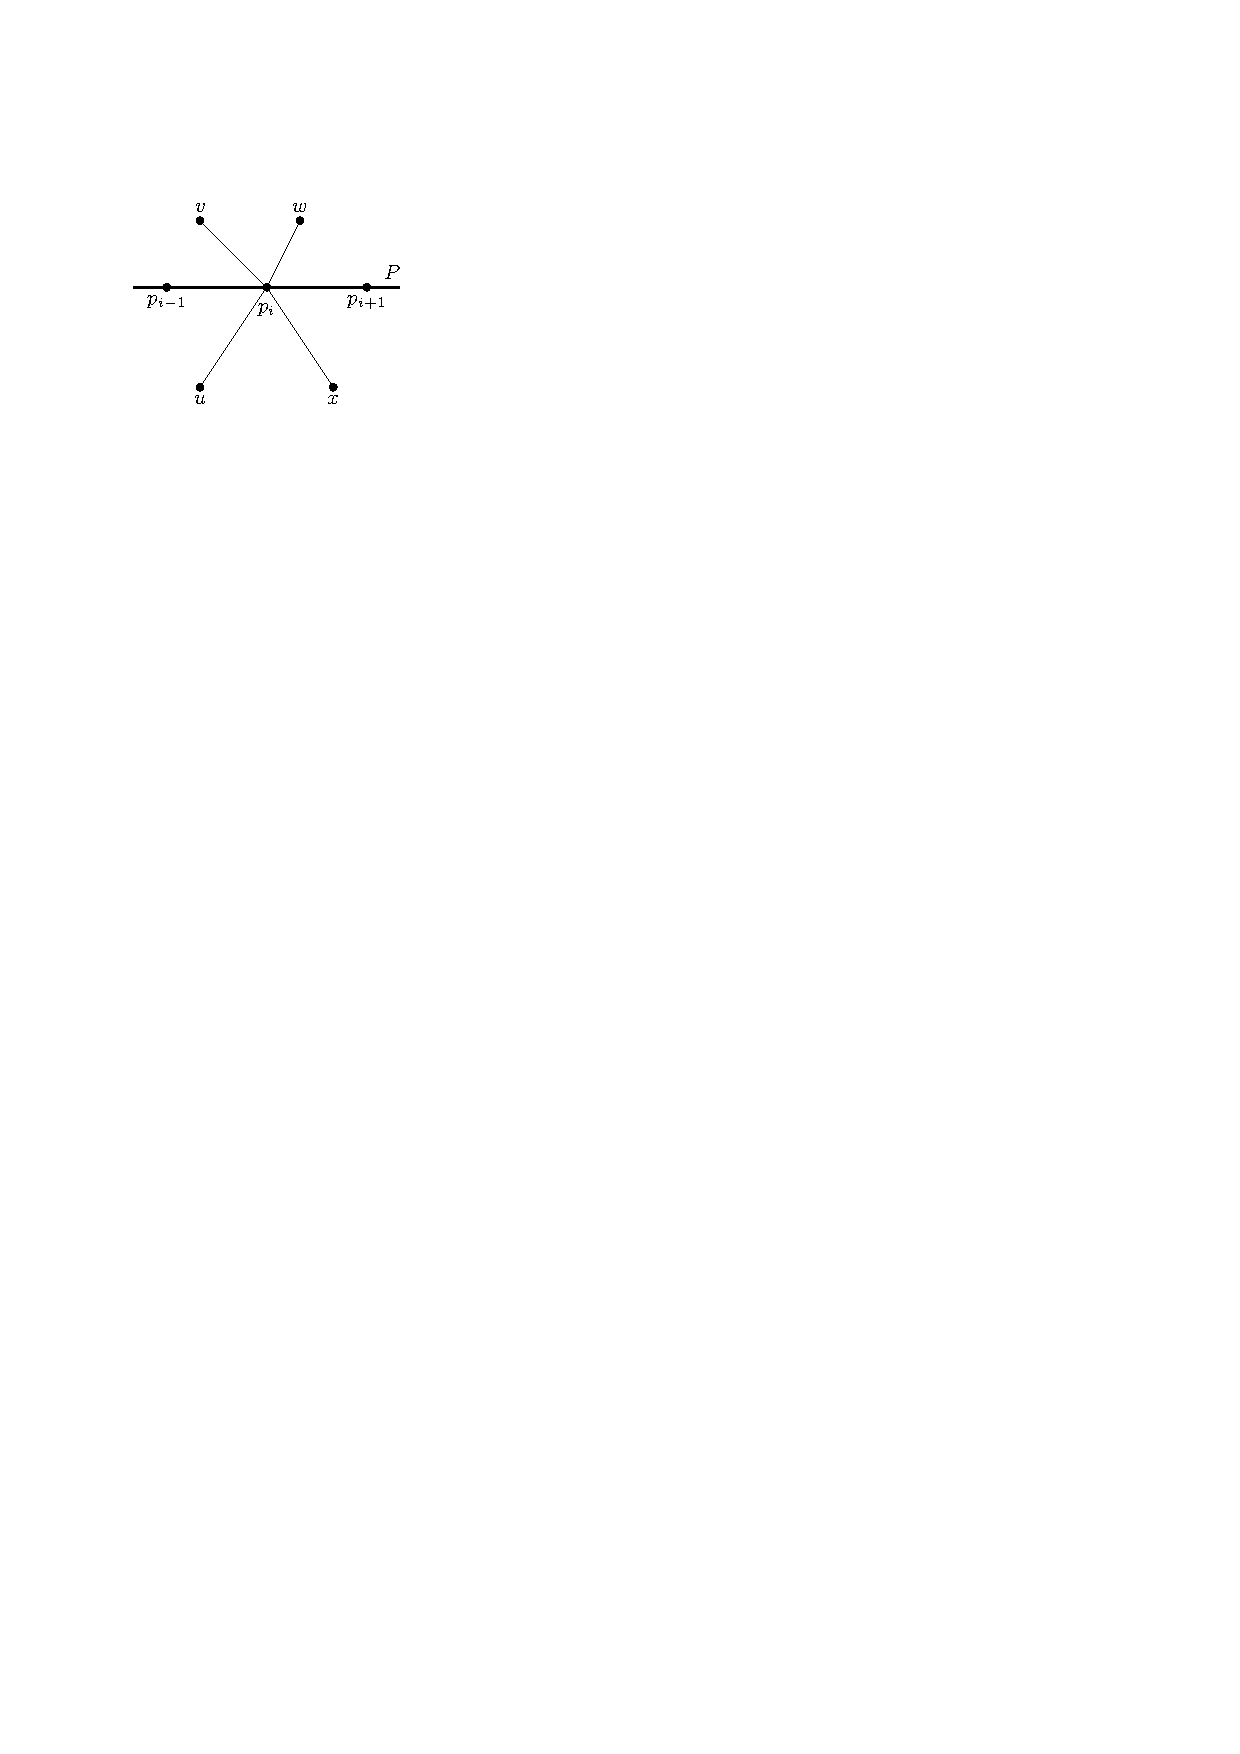
\includegraphics[scale=1]{unifiedAlgo/img/rightNeighbourwalk/rotation}
      \caption{}
      \label{fig:right:rot}
    \end{figure}

  \mypar{Path manipulations}
    With $\rev{P}$ we denote the \emph{reversed path} $p_k \ldots p_1$. We use $\oplus$ to denote the \emph{concatenation} of paths. That is, given a second path $\Q$ with vertices $q_1 \ldots q_l$ and $p_k = q_1$ the path $\P \oplus \Q$ consists of $p_1 \ldots p_{k-1} q_1 q_2 \ldots q_l$.
    Recall that a cycle is simply a path starting and ending at the same vertex. Hence if we have two  internally disjoint paths $\P, \Q$ from $s$ to $t$ then $\P \oplus \rev{\Q}$ is a cycle.
    Furthermore we use a vertical bar to denote the \emph{restriction} of a path to a certain set of vertices. So $\P|_{p_i, p_j}$ with $i<j$ is the subpath of $\P$ with vertices $p_i \ldots p_j$.

  \mypar{Chords}
    A \emph{chord} of a path is an edge that connects two non-subsequent vertices. A path without chords is \emph{chordfree}. The path $P$ in Figure \ref{fig:right:chord} has the chord $p_1 p_3$.
    A \emph{k-chord} is a path $Q$ of length $k$ that connects two non-subsequent vertices $p_i, p_j$ of $P$ such that $P \cap Q = \braces{p_i, p_j}$.
    Note that $\P|_{v_i, v_j} \oplus \rev{\Q}$ is a cycle.
    A ($k$-)chord $Q$ is \emph{separating} if this cycle is separating. In Figure \ref{fig:right:chord} there are two $2$-chords, $p_3 u p_5$ and $p_3 v p_5$, but only one of them is separating, namely $p_3 v p_5$.
    Since a cycle is a special type of path the same definitions apply to them.

    \begin{figure}[h]
      \centering
      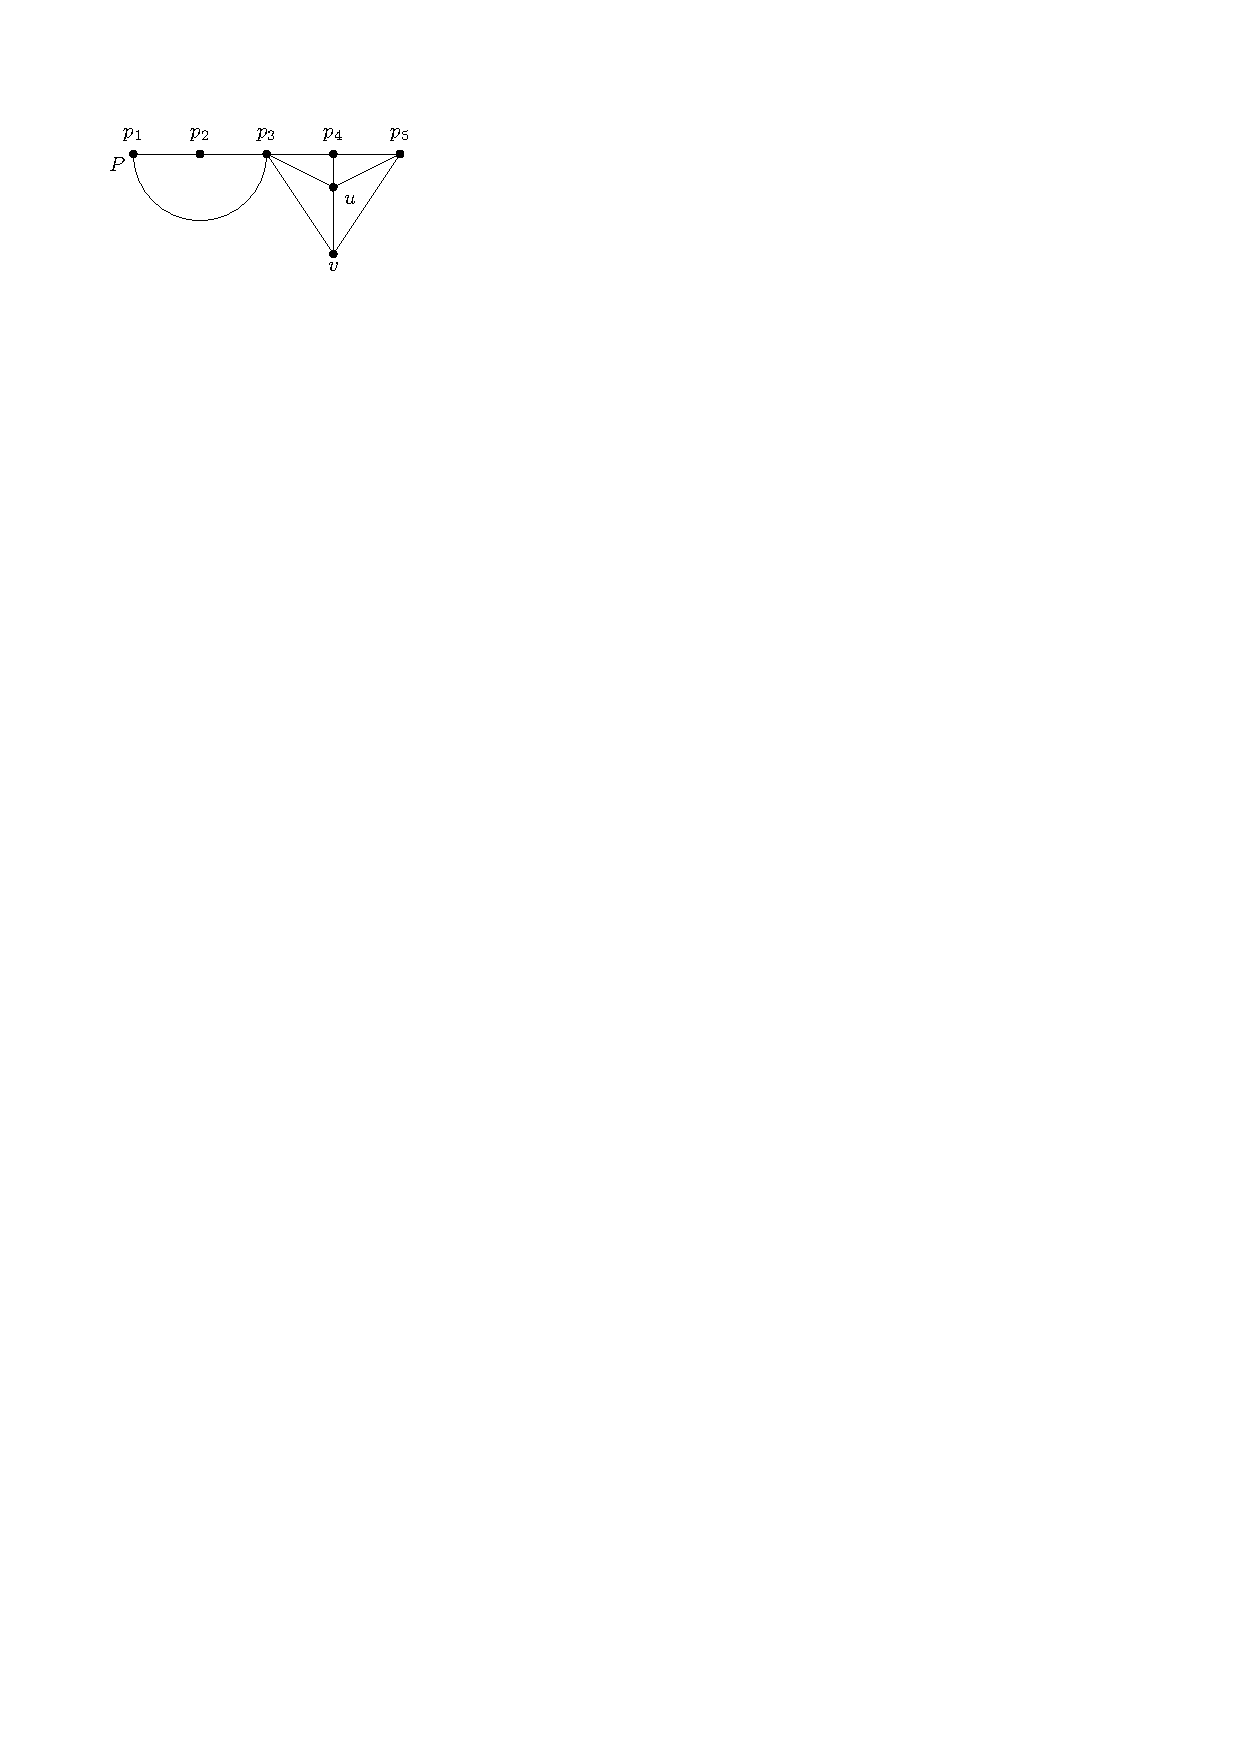
\includegraphics[scale=1]{unifiedAlgo/img/rightNeighbourwalk/chords.pdf}
      \caption{A path with a chord and a separating 2-chord}
      \label{fig:right:chord}
    \end{figure}

  \mypar{Right neighbor paths}
    We already mentioned that in the sweepcycle step we use the right neighbor path of a path. Recall that  $P$ has no interior vertices incident to the outer face and no chords or separating 2-chords on the right. We first show that every vertex has right neighbours, then we give the procedure for making the right neighbor path. Afterwards we show that the right neighbour path is a walk (Lemma \ref{lm:right:neighborWalk}) and a path (Lemma \ref{lm:right:neighborPath}).

    \begin{lemma}
      \label{lm:right:pHasRightNeihgbours}
      Every interior vertex of $P$ has at least one neighboring vertex on the right.
    \end{lemma}

    \begin{proof}
      Suppose that a interior vertex $p_i$ has no neighbor on the right of the path. Then $ \ldots p_{i-1} p_i p_{i+1} \ldots $ is a partial face border. Since $p_i$ is not incident to the outer face $p_i$ must be incident to a face of degree $3$. Thus $p_{i-1} p_i p_{i+1}$ is a face. However, this would imply a chord on the right of $P$ as can be seen in Figure \ref{fig:right:pHasRightNeighbor}. Hence by contradiction $p_i$ must have a neighbor on the right.
    \end{proof}

    \begin{figure}[h]
      \centering
      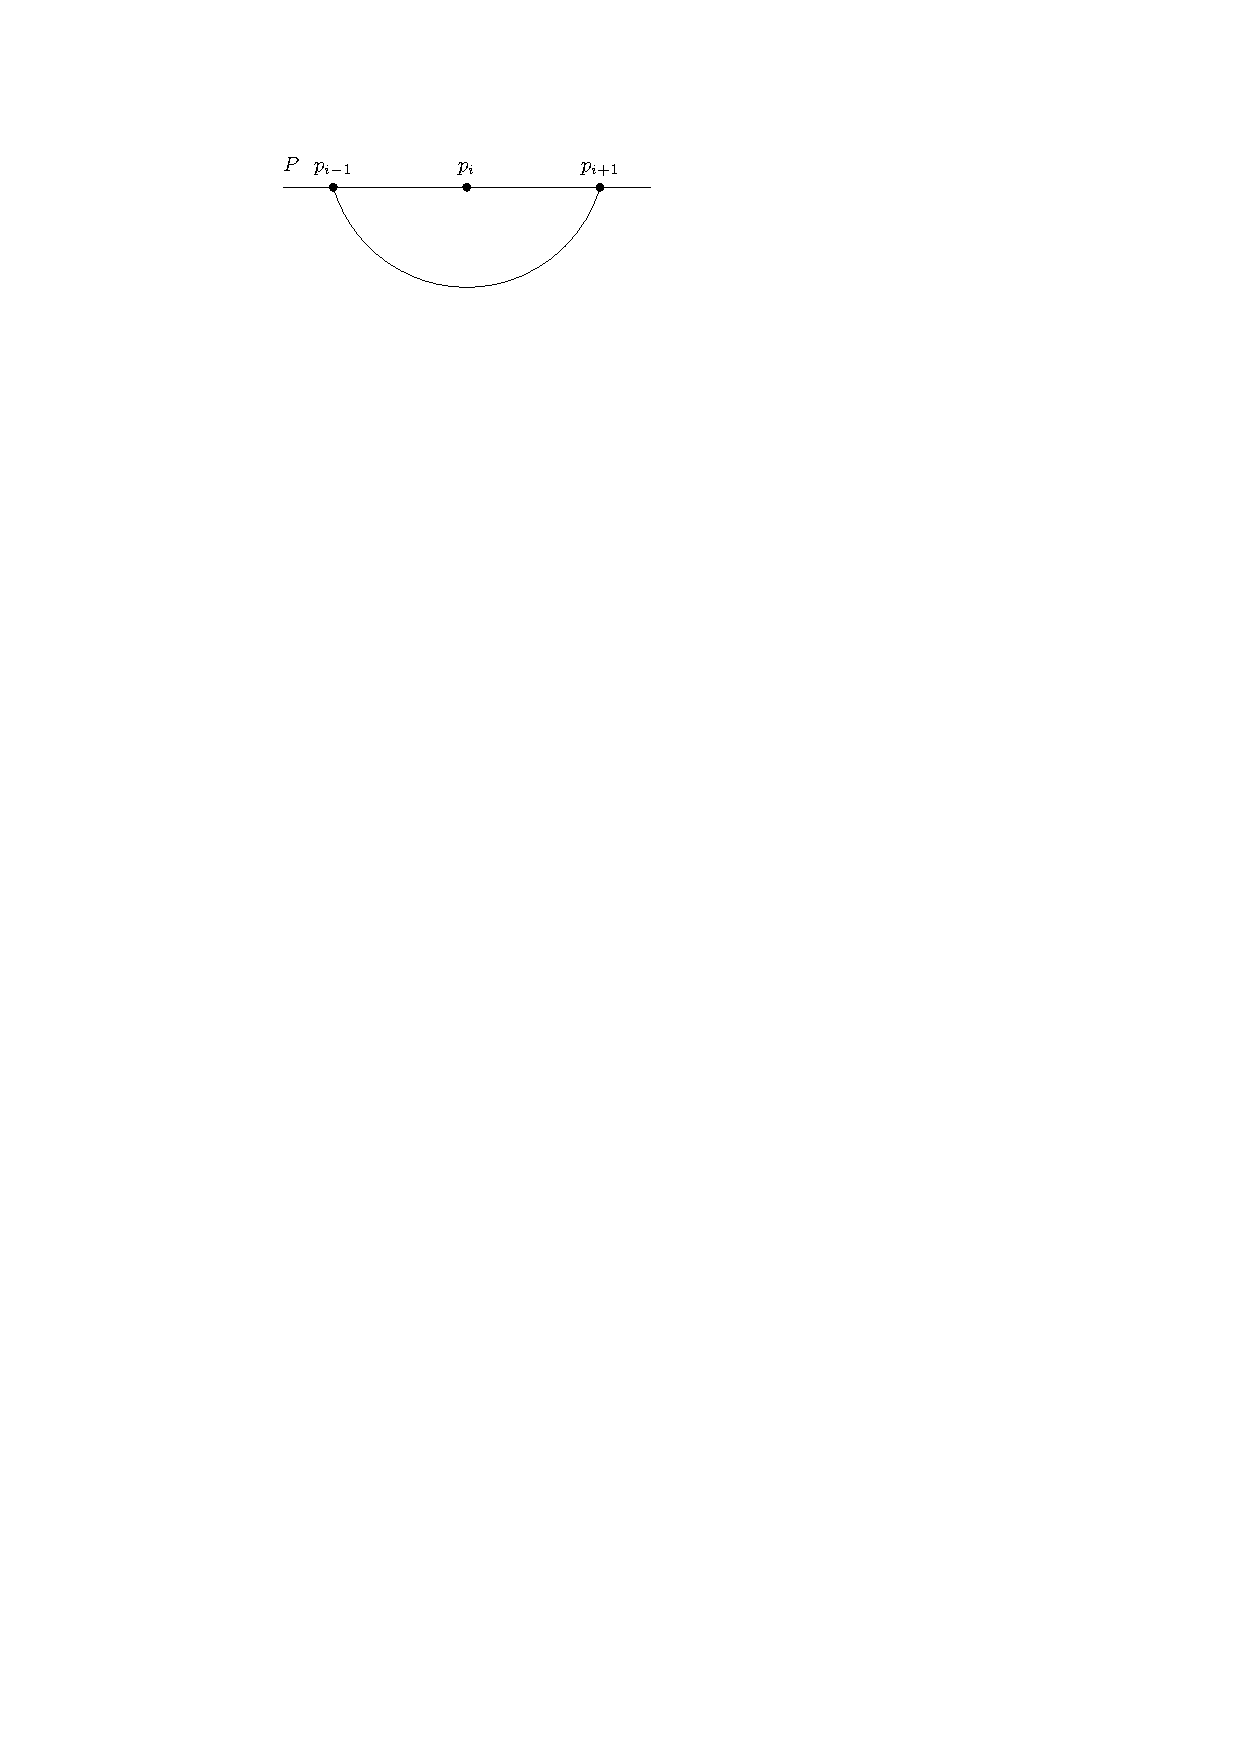
\includegraphics[scale=1]{unifiedAlgo/img/rightNeighbourwalk/pHasRightNeighbor.pdf}
      \caption{}
      \label{fig:right:pHasRightNeighbor}
    \end{figure}

    These right neighbors of $P$ will form the the \emph{right neighbor path} $Q$ of $P$.
    Let us first define a larger list of vertices $Q'$. $Q'$ will consist of $p_1$ and those vertices adjacent to $p_{2}$ that are in the exclusive interval $(p_1, p_3)$ of the clockwise rotation at $p_2$. Followed by the vertices in the interval $(p_2, p_4)$ of the rotation at $p_{3}$. We continue this up to the vertices in the interval $(p_{k-2}, p_k)$ of the rotation at $p_{k-1}$ and finally $p_k$.
    We obtain $Q$ from $Q'$ by removing all subsequent duplicates from $Q$.
    In Figure \ref{fig:right:neighborPath} an example of a right neighbor path is given.

    \begin{figure}[h]
      \centering
      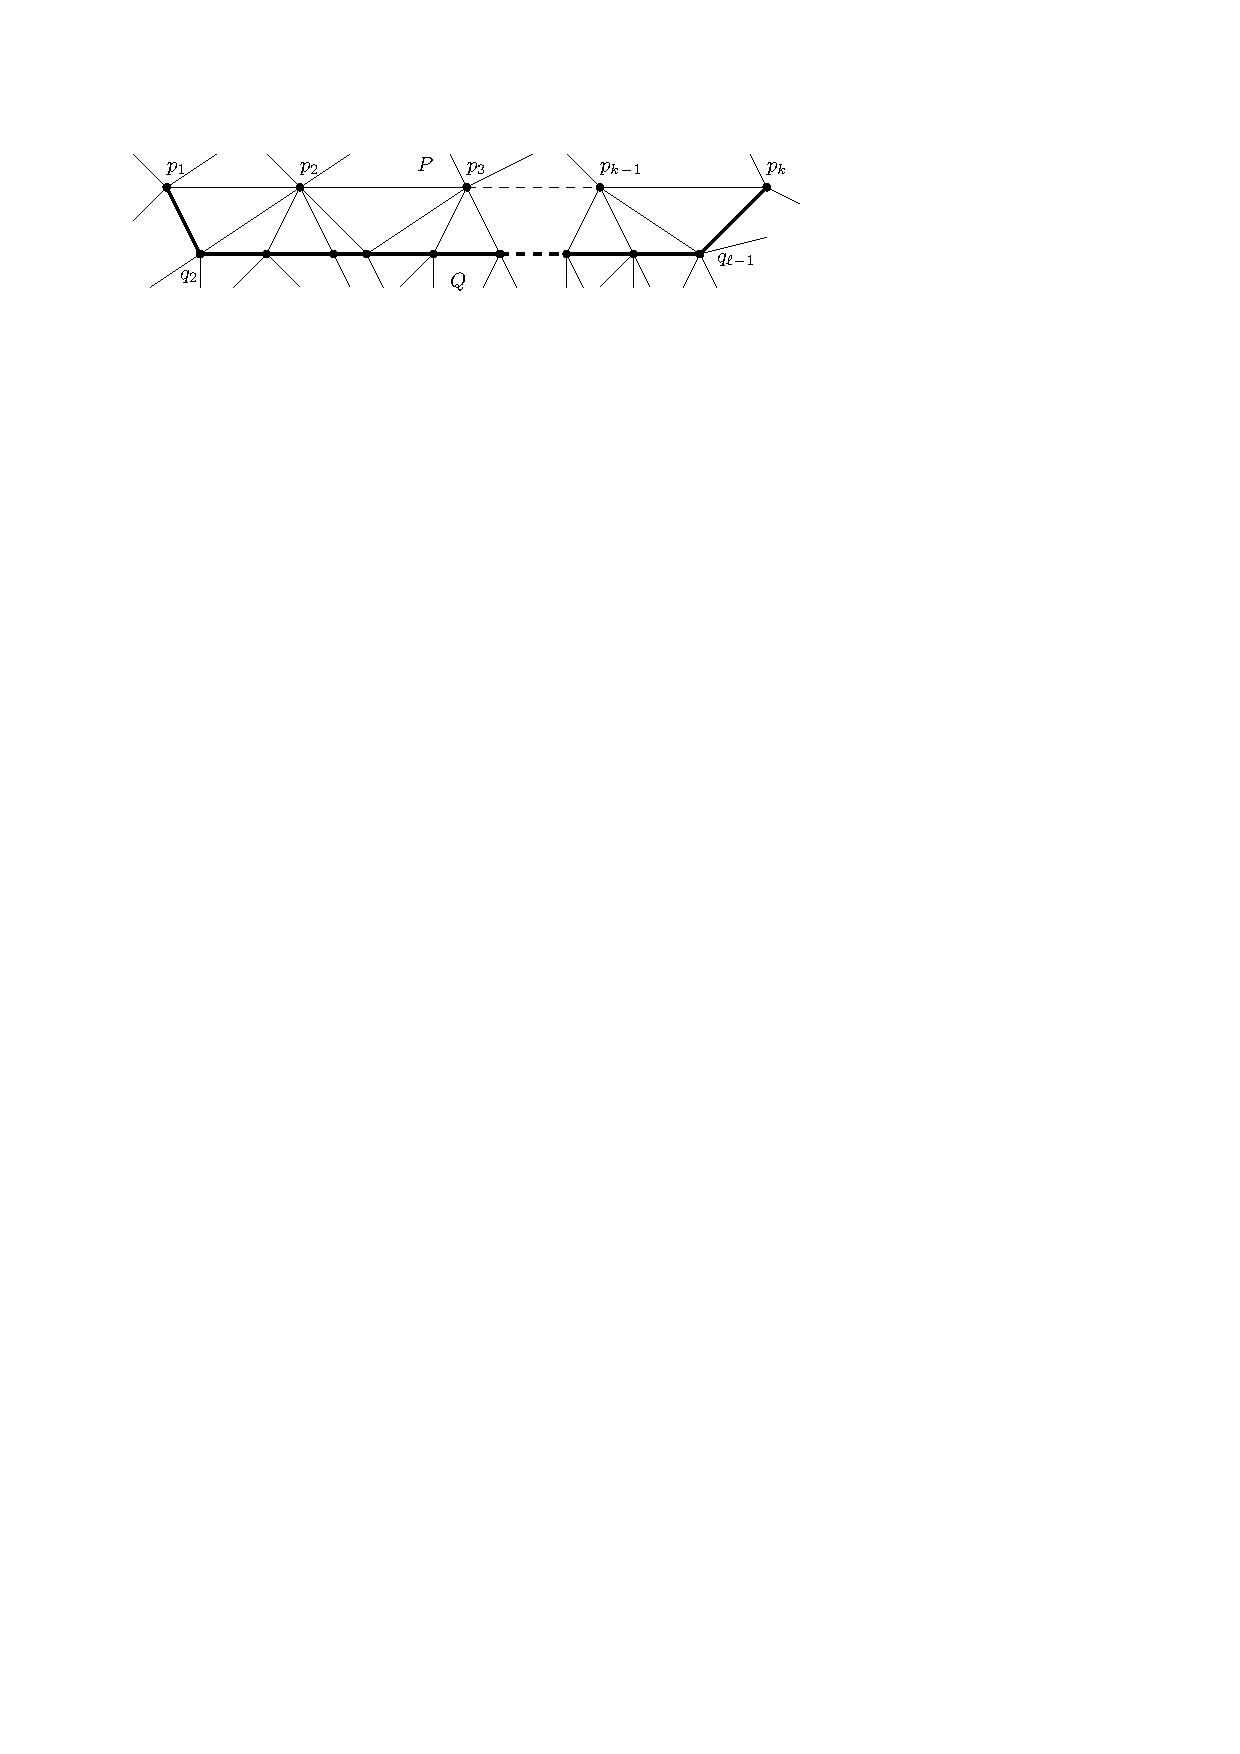
\includegraphics[scale=1]{unifiedAlgo/img/rightNeighbourwalk/neighborPath.pdf}
      \caption{}
      \label{fig:right:neighborPath}
    \end{figure}

    To break the proof that $Q$ is a path into two parts we define a \emph{walk} as a path without the constraint to be simple. Hence a walk is a sequence of vertices that are connected to each other but vertices may repeatedly occur.
    \begin{lemma}
      \label{lm:right:neighborWalk}
      The right neighbor path $Q$ is a walk.
    \end{lemma}
    \begin{proof}
      Let us denote the vertices of $Q$ by $q_1 q_2 \ldots q_\ell$.
      Let $q_i$ and $q_{i+1}$ be two subsequent vertices of $Q'$. We will show they are either connected or the same vertex. We first consider the case where $1 < i < \ell-1$.
      Now there are two sub-cases. Either $(a)$ $q_i$ and $ q_{i+1}$ are vertices adjacent to the same vertex $p_j$ an thus subsequent in the rotation at $p_j$ or $(b)$ $q_i$ was the last vertex adjacent to $p_j$ and thus $q_{i+1}$ is the first vertex adjacent to $p_{j+1}$ since by Lemma \ref{lm:right:pHasRightNeihgbours} every interior vertex of $P$ has right neighbors.
      Both cases are depicted in Figure \ref{fig:uni:walkproof}

      In case $(a)$ we note that since $q_i$ and $q_{i+1}$ are subsequent in the rotation at $p_j$ $q_i q_{i+1}$ is an edge since $p_j$ is not incident to the outer face and every interior face of $G$ is a triangle.

      In case $(b)$ we note that $p_i q_i$ and $p_i p_{i+1}$ are edges subsequent in clockwise order, hence $q_{i} p_{i+1}$ is also an edge. Hence $q_i$ is the first vertex adjacent to $p_{i+1}$ subsequent to $v_i$ in the clockwise rotation. Thus $q_{i} = q_{i+1}$. They are duplicates.

      Now for the cases $i=1$ and $i=k-1$. $q_1$ and $q_2$ are vertices adjacent to $p_{2}$ subsequent in the clockwise rotation of ${p_2}$ and hence connected since every interior face is a triangle. In the same way $q_{k-1}$ and $q_k$ are subsequent vertices in the rotation at $q_{k-1}$ and hence connected. This can also be seen in Figure \ref{fig:right:neighborPath}.

      Since all pairs of subsequent vertices in $Q'$ are connected or duplicates the step removing all duplicates from $Q'$ ensures $Q$ is a walk.

      \begin{figure}[b]
        \centering
        \begin{subfigure}[b]{0.5\linewidth}
            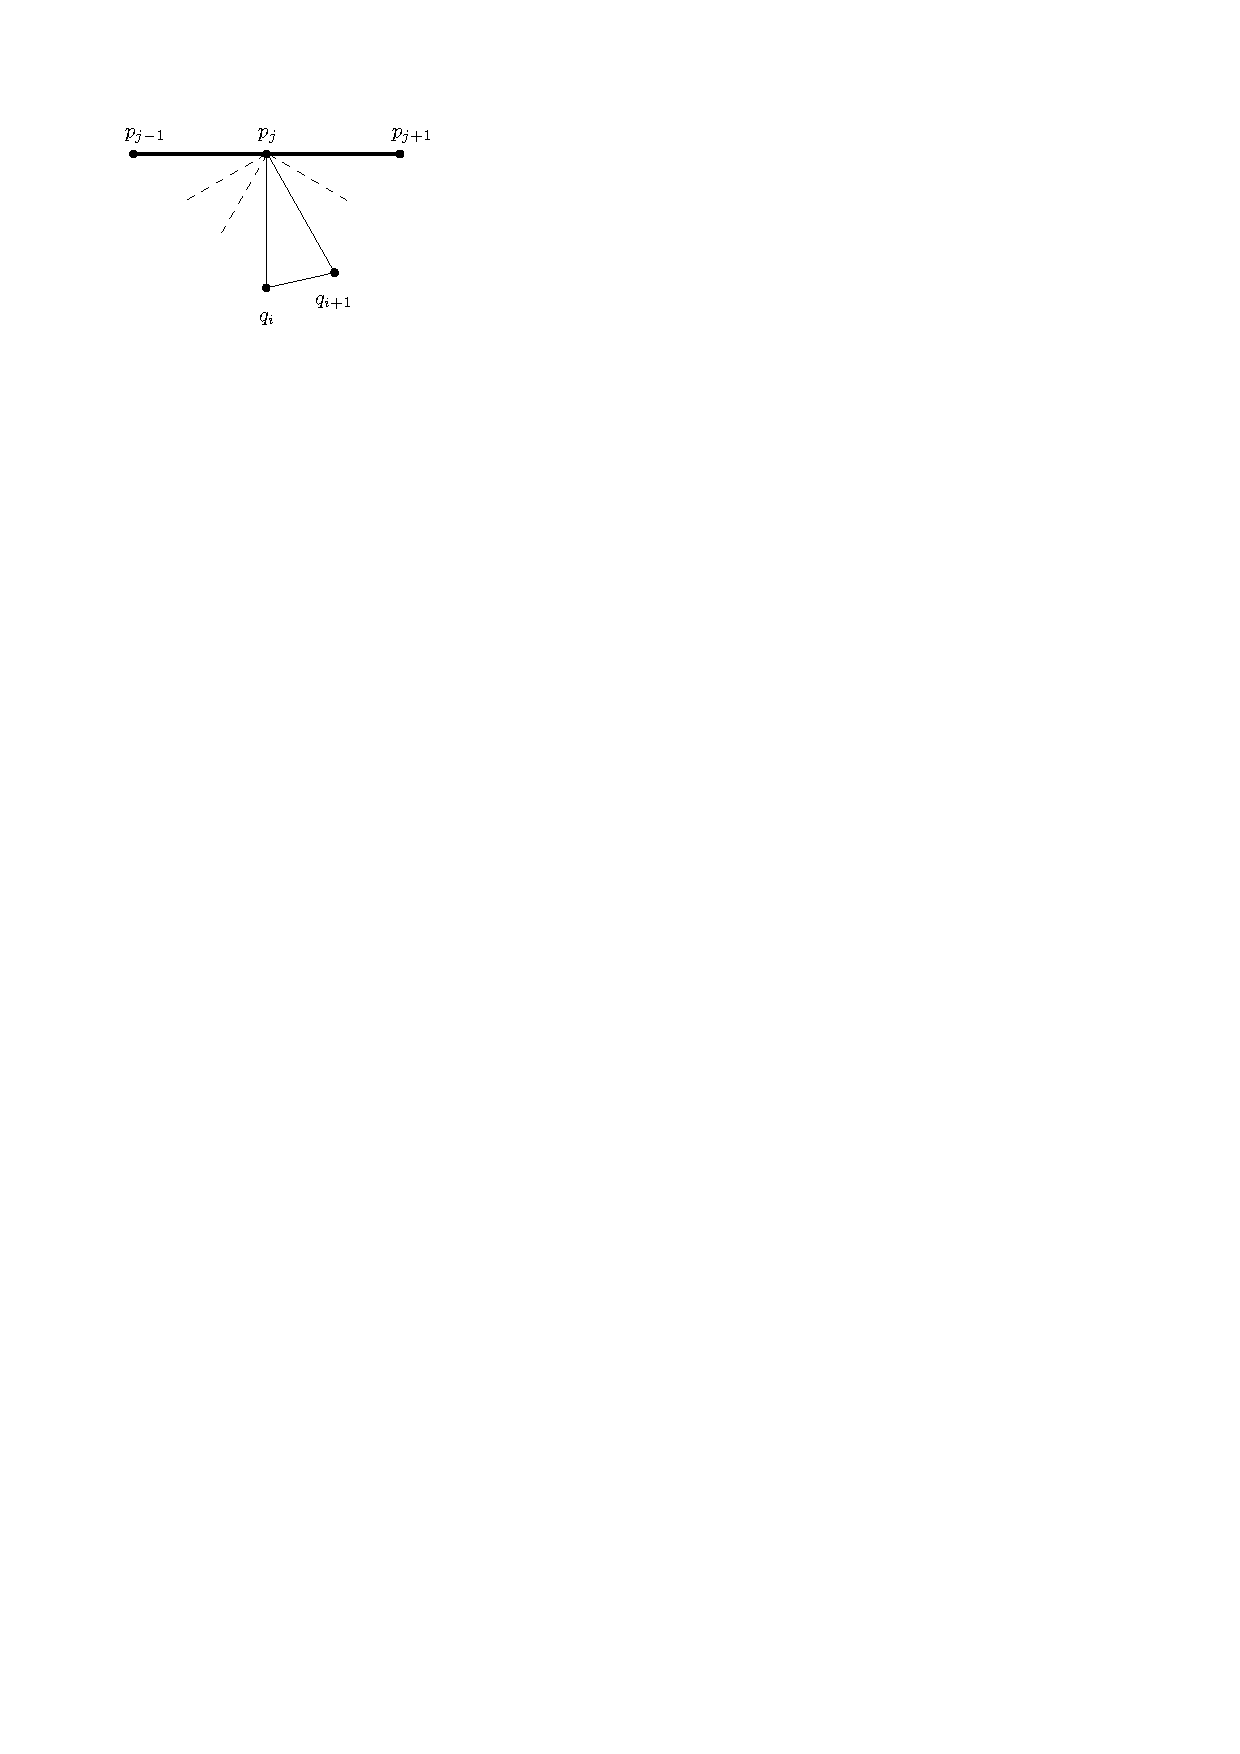
\includegraphics[width=\linewidth]{unifiedAlgo/img/walkProofA}
            \caption{}
        \end{subfigure}%
        \begin{subfigure}[b]{0.5\linewidth}
            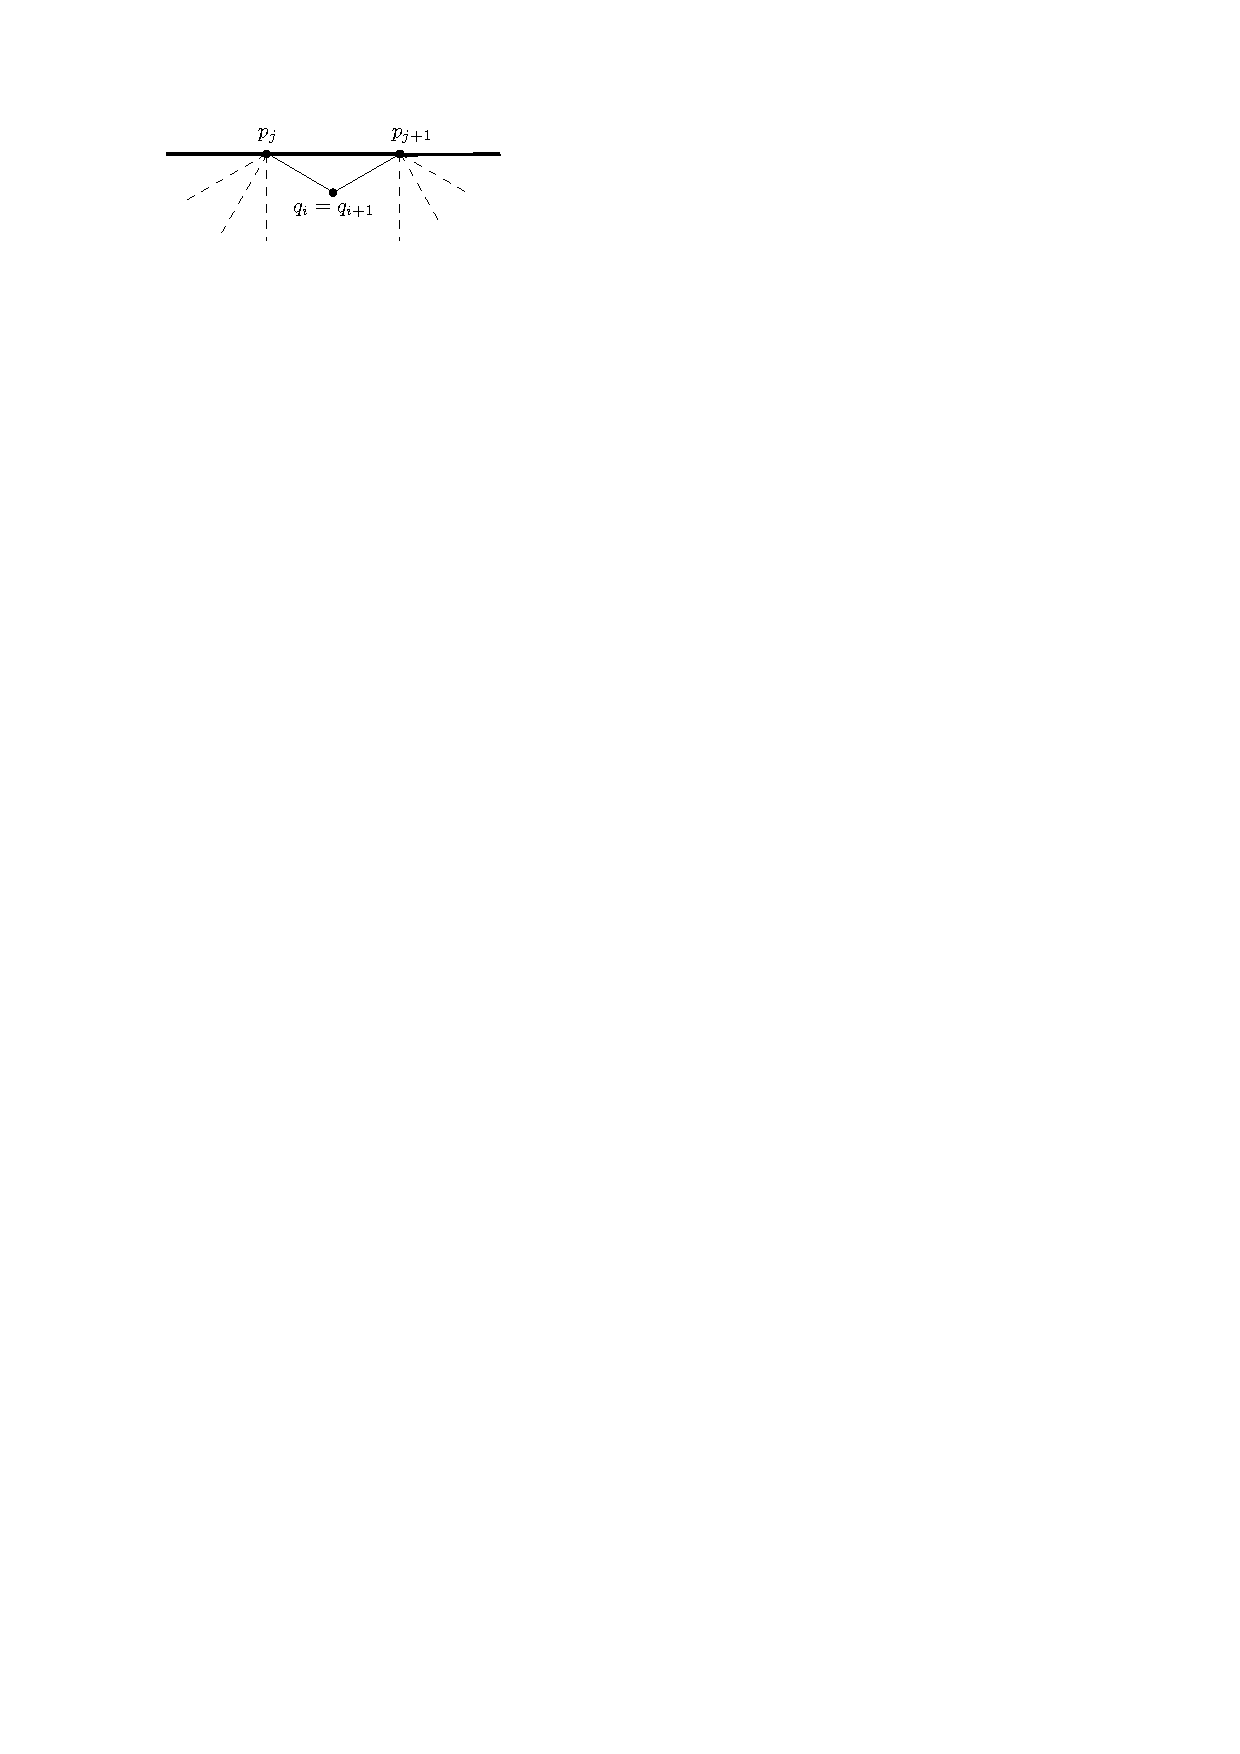
\includegraphics[width=\linewidth]{unifiedAlgo/img/walkProofB}
            \vspace{1cm}
            \caption{}
        \end{subfigure}
        \caption{The two main cases of the proof showing that $W$ is a walk}
        \label{fig:uni:walkproof}
      \end{figure}
    \end{proof}

    \begin{lemma}
      \label{lm:right:neighborPath}
      The right neighbor path $Q$ is a path
    \end{lemma}
    \begin{proof}
      We already know $Q$ is a path by \ref{lm:right:neighborWalk}. Hence we only have to show that $Q$ contains no duplicate vertices.

      Suppose that $Q$ has a duplicate vertex $q_i=q_j$ with $i<j$. Then this vertex must have been a neighbor to two different vertices in $P$. We denote these vertices $p_\ell$, $p_k$ with $\ell<k$. We are now in the situation of Figure \ref{fig:right:path}.

      By the order in which we added vertices to $Q'$, which is preserved by the removal of when we go to $Q$, we know that any vertices in-between $q_i$ and $q_j$ in $Q$ must be one of the following:
      \begin{enumerate}
        \item Adjacent to $p_\ell$ and in the interval $(q_i, p_{\ell+1})$ in $p_\ell$'s rotation.
        \item Adjacent to one of $p_{\ell+1},  p_{\ell+2},\ldots, p_{k-1}$ and to the right of $P$.
        \item Adjacent to $p_k$ and in the interval $(p_{k-1}, q_j)$ in $p_k$'s rotation.
      \end{enumerate}


      All three cases describe a vertex that lies in the interior of the cycle $q_i p_i p_{i+1} \ldots p_j$. However, since $P$ has no separating $2$-chords on the right this cycle must be empty. Therefore there are no vertices in-between $q_i$ and $q_j$. But $Q$ is a walk and $G$ is simple  so $Q$ has no subsequent duplicates. Hence $Q$ contains no duplicates at all and is thus a path.
    \end{proof}

    \begin{figure}[h]
      \centering
      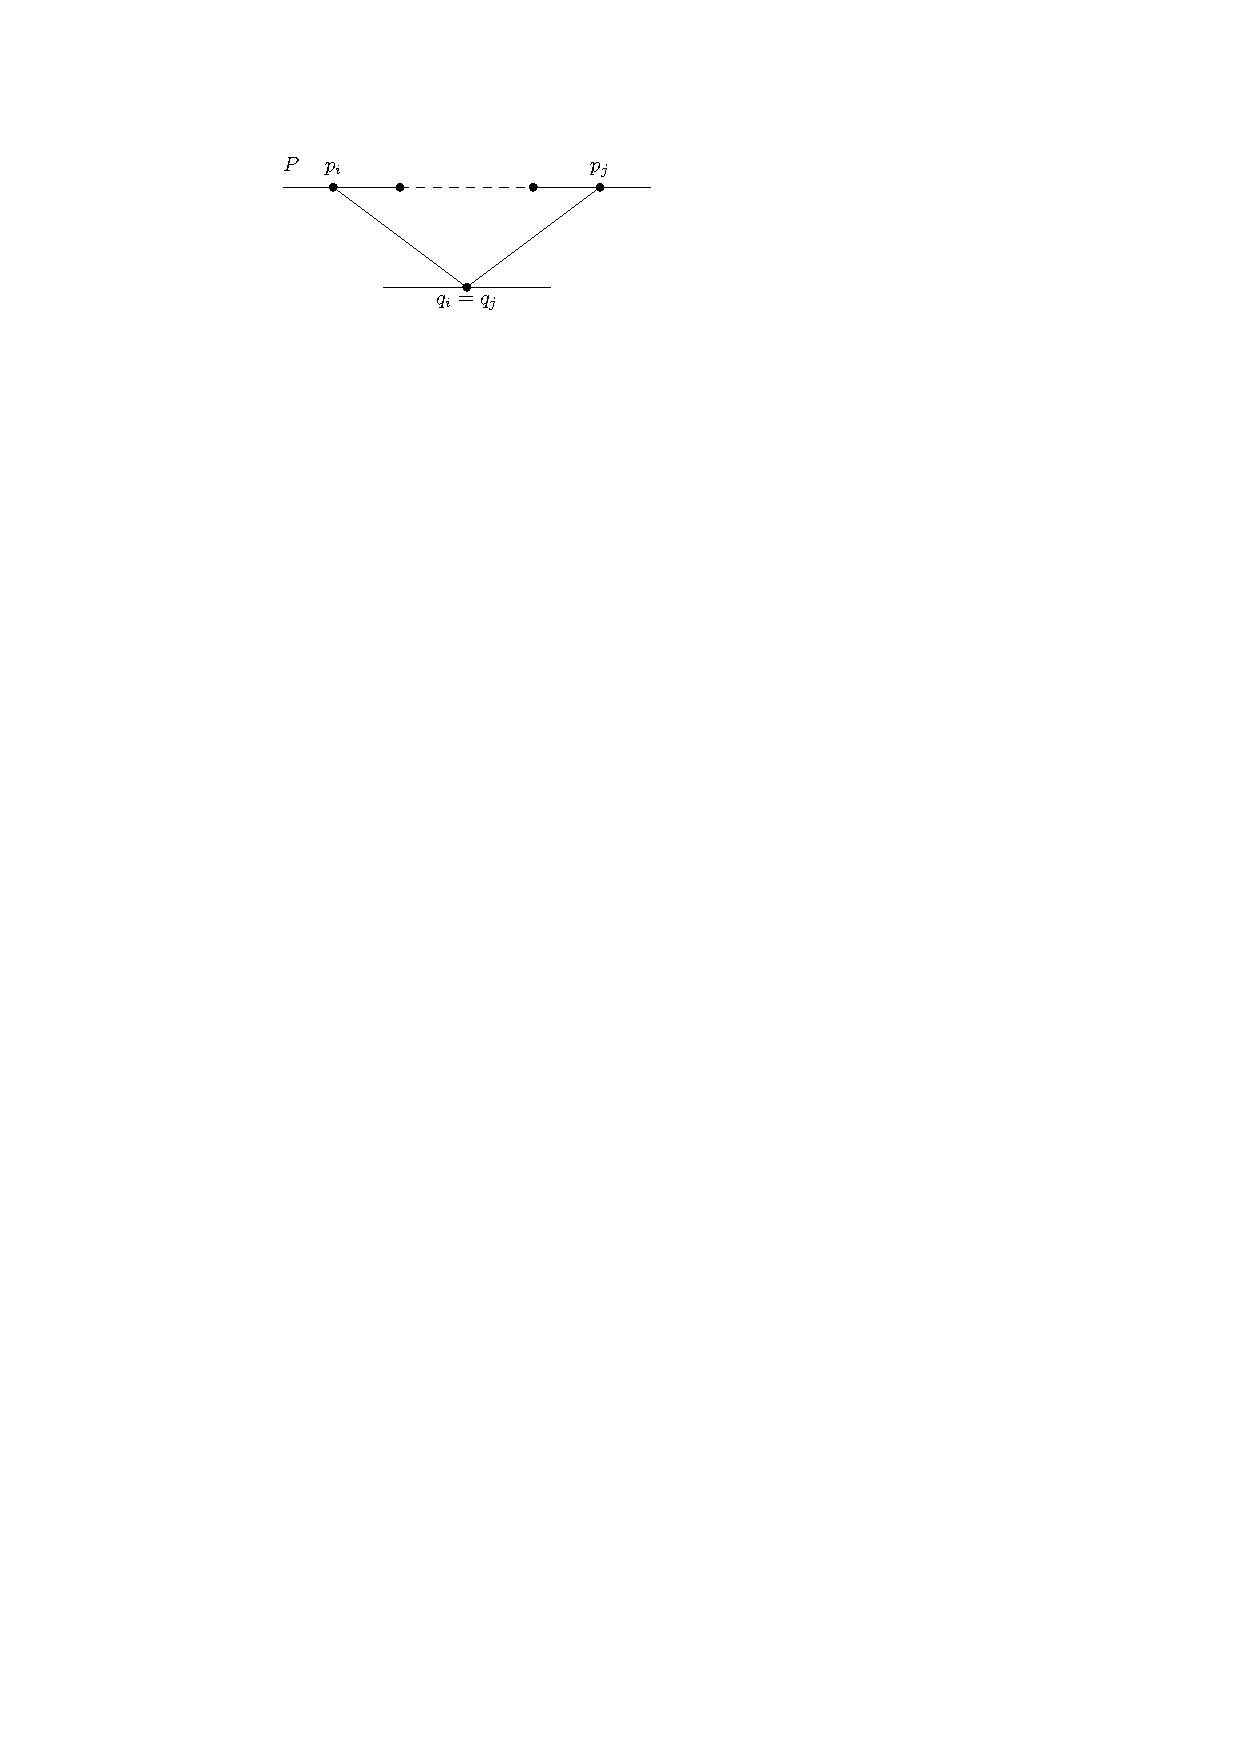
\includegraphics[scale=1]{unifiedAlgo/img/rightNeighbourwalk/neighborPathisPath.pdf}
      \caption{}
      \label{fig:right:path}
    \end{figure}

    \begin{lemma}
      \label{lm:right:neighbourwalkNoInteriorVertex}
      The cycle $P \oplus \rev{Q}$ has no interior vertices.
    \end{lemma}
    \begin{proof}
      In the construction of the right neighbor path both cases in Figure \ref{fig:uni:walkproof} add a triangle to the interior with all vertices of the triangle in $W \oplus \rev{P}$. Hence the interior of $P \oplus \rev{Q}$ can be subdivided in a number triangles.

      Suppose there is a interior vertex in the cycle $P \oplus \rev{Q}$. Then the triangle containing this vertex is a separating triangle. Hence $P \oplus \rev{Q}$ has no interior vertices.
    \end{proof}


    \begin{lemma}
      \label{lm:right:neighbourwalkChordFree}
      The left of a right neighbor path is chordfree.
    \end{lemma}
    \begin{proof}
      Suppose that the right neighbor path $Q = q_1 \ldots q_k$  has a chord on the left, say an edge between $q_i$ and $q_j$ with $i< j -1 $. There is a vertex $p_\ell \in P$ on the path such that $q_{i+1}$ is a neighbor of $p_\ell$ to the left of $p_\ell$. Consider now the cycle $P q_k \ldots q_{j+1} q_j q_i q_{i-1} \ldots q_1$
      (thick in Figure \ref{fig:uni:neihbourwalkChordFree}) this cycle has $q_{i+1}$ in its exterior. But then $p_\ell w_{i+1}$ is a crossing edge, which is forbidden.
      \fxwarning{TODO argue that an edge in the exterior is also imposible usning the path $P$. Maybe the vertex $q_{i+1}$ is actually in some cycle}

      \begin{figure}[h]
        \centering
        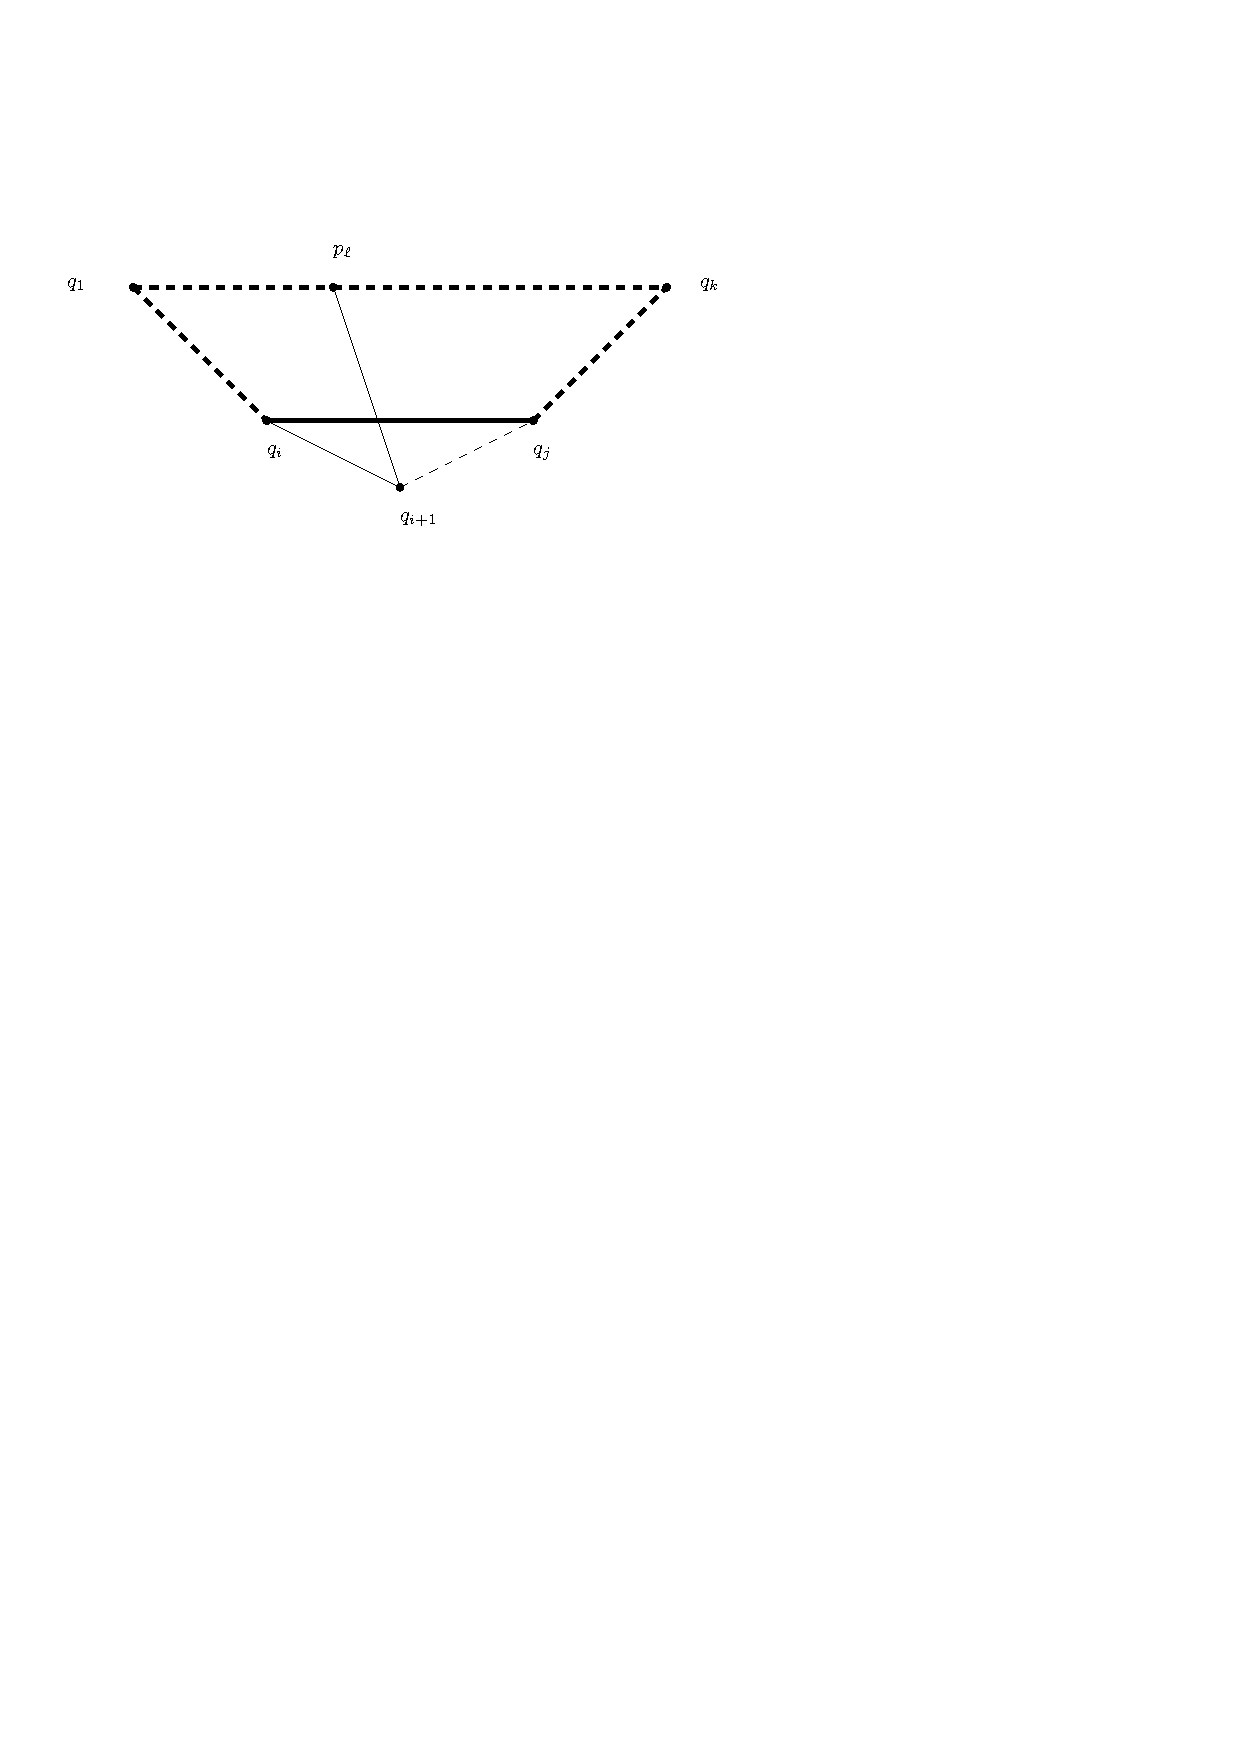
\includegraphics[scale=1]{unifiedAlgo/img/neighbourWalkChords}
        \caption{The construction in the proof of Lemma \ref{lm:right:neighbourwalkChordFree}}
        \label{fig:uni:neihbourwalkChordFree}
      \end{figure}
    \end{proof}
